\section{USGS ScienceBase}

To facilitate and encourage data sharing and dissemination,
the U.S. Geological Survey has created ScienceBase, an online
collaborative scientific data platform (Figure \ref{figure:sbfig}).
ScienceBase is targeted for use by USGS researchers, their collaborators, 
and the end users of reviewed and released USGS data products.
ScienceBase has four key elements to support collaborative
data workflows: 1) Data and metadata
cataloging and hosting with options for private, controlled access
and fully public sharing of data and metadata. 2) Central search and
data discovery for both data hosted on ScienceBase and externally hosted 
data. 3) Full web-service support for all core functionality, including
standards-based access to specific data types (e.g.\ geospatial
datasets). 4) Research community catalogs to
enable the organization of data along collaborative group and
organizational boundaries.

 \begin{figure}[htbp]
   \centering
   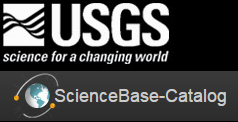
\includegraphics{sblogo}
   \caption{The ScienceBase platform logo}
   \label{figure:sbfig}
 \end{figure}

ScienceBase users store data in 'items', where each item is a flexible
representation of a dataset and its metadata. The dataset component of an
item can be one or more data files in any format or simply an item with descriptive
metadata linking a dataset hosted on an external repository. This supports
indexing of legacy datasets that are hosted in well known locations (for example, 
the USGS National Hydrography Dataset). Items are organized into a tree hierarchy 
(much like the structure of files and
folders on a hard drive). This allows data to be intuitively organized by the
institution, collaborative group, and/or individual to whom
the data belong. At the same time, items can also be assigned identifying tags
for rapid search and data discovery across the full ScienceBase catalog.

Search and management of ScienceBase data items can be accomplished through
both graphical and scripted interfaces. Manual search, data upload/download, and
metadata editing are possible through the ScienceBase website.
Automated access to all of these functions is supported by robust RESTful web
services and a documented API. The ScienceBase code and infrastructure setup 
is available upon request from the ScienceBase team <sciencebase@usgs.gov>. 
Further information and details can be found in the online 
\href{https://www.sciencebase.gov/about/using-sciencebase}{ScienceBase Documentation}.
